\documentclass[aspectratio=169,11pt]{beamer}
\usetheme{Madrid}
\usecolortheme{seahorse}
\usefonttheme{structurebold}

\usepackage{listings}
\usepackage{xcolor}
\usepackage{tikz}
\usepackage{booktabs}
\usepackage{pifont}
\usepackage{amssymb}
\usepackage{multicol}

% SQL Syntax Highlighting
\lstdefinestyle{sqlstyle}{
    language=SQL,
    basicstyle=\ttfamily\scriptsize,
    keywordstyle=\color{blue!70!black}\bfseries,
    stringstyle=\color{red!60!black},
    commentstyle=\color{green!50!black}\itshape,
    numbers=left,
    numberstyle=\tiny\color{gray},
    numbersep=5pt,
    frame=single,
    backgroundcolor=\color{gray!10},
    breaklines=true,
    showstringspaces=false,
    tabsize=2,
    morekeywords={DATABASE, REFERENCES, LIMIT, OFFSET, CASCADE, RESTRICT, 
                  AUTO_INCREMENT, IDENTITY, SERIAL, RETURNING, ILIKE,
                  RANK, DENSE_RANK, ROW_NUMBER, PARTITION, OVER, LAG, LEAD,
                  FIRST_VALUE, LAST_VALUE, NTH_VALUE, CUBE, ROLLUP, GROUPING SETS,
                  WITH, RECURSIVE, CTE, WINDOW, FRAME, RANGE, ROWS, UNBOUNDED,
                  PRECEDING, FOLLOWING, CURRENT ROW, EXCEPT, INTERSECT, ALL,
                  CASE, WHEN, THEN, ELSE, END, COALESCE, NULLIF, CAST, CONVERT,
                  DATE, TIME, TIMESTAMP, INTERVAL, EXTRACT, DATE_PART, NOW,
                  CURRENT_DATE, CURRENT_TIME, STRING_AGG, ARRAY_AGG, JSON_AGG,
                  XML, JSON, JSONB, HSTORE, UUID, SERIAL, BIGSERIAL, TEXT,
                  VARCHAR, CHAR, BOOLEAN, REAL, DOUBLE, NUMERIC, DECIMAL,
                  MONEY, BYTEA, BLOB, CLOB, NCLOB, XMLTYPE, CURSOR, FETCH,
                  OPEN, CLOSE, DEALLOCATE, PREPARE, EXECUTE, DEALLOCATE PREPARE}
}
\lstset{style=sqlstyle}

% Custom blocks
\setbeamertemplate{blocks}[rounded][shadow=true]

\title{Comprehensive SQL Guide}
\subtitle{From Basics to Advanced - Complete Reference with Examples}
\author{Database Systems Course}
\institute{CS Department}
\date{\today}

\begin{document}

%=============================================================================
% TITLE SLIDE
%=============================================================================
\begin{frame}
\titlepage
\end{frame}

%=============================================================================
% TABLE OF CONTENTS
%=============================================================================
\begin{frame}{Complete Roadmap}
\begin{multicols}{3}
\tableofcontents
\end{multicols}
\end{frame}

%=============================================================================
% PART 1: INTRODUCTION
%=============================================================================
\section{Introduction to SQL}

\begin{frame}{What is SQL?}
\begin{block}<1->{Definition}
\textbf{Structured Query Language (SQL)} is a domain-specific language used for managing and manipulating relational databases. It is the standard language for relational database management systems (RDBMS).
\end{block}

\pause
\begin{exampleblock}<2->{History}
\begin{itemize}
    \item Developed by IBM in the 1970s (originally called SEQUEL)
    \item First commercial implementation by Oracle in 1979
    \item ANSI standard in 1986, ISO standard in 1987
    \item Current standard: SQL:2023 (ISO/IEC 9075)
\end{itemize}
\end{exampleblock}

\pause
\begin{alertblock}<3->{Key Characteristics}
\begin{itemize}
    \item \textbf{Declarative}: You specify \textit{what} you want, not \textit{how} to get it
    \item \textbf{Set-based}: Operations work on sets of rows, not individual rows
    \item \textbf{Standardized}: Portable across different database systems (with variations)
\end{itemize}
\end{alertblock}
\end{frame}

\begin{frame}{SQL Categories}
\begin{columns}[T]
\begin{column}{0.5\textwidth}
\onslide<1->{
\begin{block}{Data Definition Language (DDL)}
Define and modify database structure:
\begin{itemize}
    \item \texttt{CREATE} - Create databases, tables, indexes
    \item \texttt{ALTER} - Modify existing structures
    \item \texttt{DROP} - Delete objects
    \item \texttt{TRUNCATE} - Remove all data
    \item \texttt{RENAME} - Rename objects
\end{itemize}
\end{block}
}

\pause
\begin{block}<2->{Data Control Language (DCL)}
Control access and permissions:
\begin{itemize}
    \item \texttt{GRANT} - Give permissions
    \item \texttt{REVOKE} - Remove permissions
    \item \texttt{DENY} - Explicitly deny access
\end{itemize}
\end{block}
\end{column}

\pause
\begin{column}{0.5\textwidth}
\begin{block}<3->{Data Manipulation Language (DML)}
Work with data:
\begin{itemize}
    \item \texttt{SELECT} - Query data
    \item \texttt{INSERT} - Add new rows
    \item \texttt{UPDATE} - Modify existing rows
    \item \texttt{DELETE} - Remove rows
    \item \texttt{MERGE} - Upsert operations
\end{itemize}
\end{block}

\pause
\begin{block}<4->{Transaction Control Language (TCL)}
Manage transactions:
\begin{itemize}
    \item \texttt{COMMIT} - Save changes
    \item \texttt{ROLLBACK} - Undo changes
    \item \texttt{SAVEPOINT} - Set savepoints
    \item \texttt{SET TRANSACTION} - Configure transaction
\end{itemize}
\end{block}
\end{column}
\end{columns}
\end{frame}

\begin{frame}{Sample Database Schema}
\begin{columns}
\begin{column}{0.6\textwidth}
\onslide<1->{
\textbf{Core Tables:}
\begin{itemize}
    \item \texttt{employees} (emp_id, first_name, last_name, email, phone, hire_date, job_id, salary, commission_pct, manager_id, dept_id)
    \item \texttt{departments} (dept_id, dept_name, location_id, manager_id)
    \item \texttt{locations} (location_id, street_address, city, state_province, country_id)
    \item \texttt{countries} (country_id, country_name, region_id)
    \item \texttt{regions} (region_id, region_name)
    \item \texttt{jobs} (job_id, job_title, min_salary, max_salary)
    \item \texttt{job\_history} (emp_id, start_date, end_date, job_id, dept_id)
\end{itemize}
}
\end{column}
\begin{column}{0.4\textwidth}
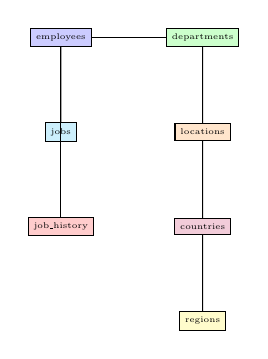
\begin{tikzpicture}[scale=0.6, transform shape]
\node[draw, fill=blue!20, rectangle, font=\tiny] (emp) at (0,0) {employees};
\node[draw, fill=green!20, rectangle, font=\tiny] (dept) at (3,0) {departments};
\node[draw, fill=orange!20, rectangle, font=\tiny] (loc) at (3,-2) {locations};
\node[draw, fill=purple!20, rectangle, font=\tiny] (cnt) at (3,-4) {countries};
\node[draw, fill=yellow!20, rectangle, font=\tiny] (reg) at (3,-6) {regions};
\node[draw, fill=cyan!20, rectangle, font=\tiny] (job) at (0,-2) {jobs};
\node[draw, fill=red!20, rectangle, font=\tiny] (hist) at (0,-4) {job\_history};

\draw (emp) -- (dept);
\draw (dept) -- (loc);
\draw (loc) -- (cnt);
\draw (cnt) -- (reg);
\draw (emp) -- (job);
\draw (emp) -- (hist);
\end{tikzpicture}
\end{column}
\end{columns}
\end{frame}

%=============================================================================
% PART 2: DATA TYPES
%=============================================================================
\section{Data Types and Constraints}

\begin{frame}{Common Data Types}
\begin{columns}[T]
\begin{column}{0.33\textwidth}
\onslide<1->{
\begin{block}{Numeric Types}
\begin{itemize}
    \item \texttt{INT/INTEGER}
    \item \texttt{BIGINT}
    \item \texttt{SMALLINT}
    \item \texttt{DECIMAL(p,s)}
    \item \texttt{NUMERIC(p,s)}
    \item \texttt{FLOAT/REAL}
    \item \texttt{DOUBLE}
    \item \texttt{SERIAL}
    \item \texttt{MONEY}
\end{itemize}
\end{block}
}
\end{column}

\pause
\begin{column}{0.33\textwidth}
\begin{block}<2->{Character Types}
\begin{itemize}
    \item \texttt{CHAR(n)} - Fixed
    \item \texttt{VARCHAR(n)} - Variable
    \item \texttt{TEXT} - Unlimited
    \item \texttt{NCHAR(n)} - Unicode
    \item \texttt{NVARCHAR(n)}
    \item \texttt{CLOB} - Large text
    \item \texttt{NCLOB}
\end{itemize}
\end{block}
\end{column}

\pause
\begin{column}{0.33\textwidth}
\begin{block}<3->{Date/Time Types}
\begin{itemize}
    \item \texttt{DATE}
    \item \texttt{TIME}
    \item \texttt{TIMESTAMP}
    \item \texttt{DATETIME}
    \item \texttt{INTERVAL}
    \item \texttt{YEAR}
    \item \texttt{YEAR TO MONTH}
    \item \texttt{DAY TO SECOND}
\end{itemize}
\end{block}
\end{column}
\end{columns}

\pause
\vspace{0.3cm}
{\scriptsize
\textbf{Example:} \texttt{CREATE TABLE products (product\_id SERIAL PRIMARY KEY, product\_name VARCHAR(100) NOT NULL, price DECIMAL(10,2) CHECK (price > 0), quantity INT DEFAULT 0, description TEXT, created\_at TIMESTAMP DEFAULT CURRENT\_TIMESTAMP);}
}
\end{frame}

\begin{frame}{Constraints}
\begin{columns}[T]
\begin{column}{0.5\textwidth}
\onslide<1->{
\begin{block}{Column Constraints}
\begin{itemize}
    \item \texttt{NOT NULL} - Must have value
    \item \texttt{UNIQUE} - No duplicates
    \item \texttt{PRIMARY KEY} - Unique + Not Null
    \item \texttt{FOREIGN KEY} - References another table
    \item \texttt{CHECK} - Custom condition
    \item \texttt{DEFAULT} - Default value
    \item \texttt{AUTO_INCREMENT} - Auto number
\end{itemize}
\end{block}
}
\end{column}

\pause
\begin{column}{0.5\textwidth}
\begin{exampleblock}<2->{Constraint Examples}
{\scriptsize
\begin{verbatim}
CREATE TABLE orders (
    order_id INT PRIMARY KEY,
    customer_id INT NOT NULL,
    order_date DATE DEFAULT 
        CURRENT_DATE,
    total_amount DECIMAL(10,2) 
        CHECK (total_amount >= 0),
    status VARCHAR(20) DEFAULT 
        'Pending',
    CONSTRAINT fk_customer
        FOREIGN KEY (customer_id)
        REFERENCES customers(id)
        ON DELETE CASCADE
);
\end{verbatim}
}
\end{exampleblock}
\end{column}
\end{columns}
\end{frame}

%=============================================================================
% PART 3: DDL - DATA DEFINITION
%=============================================================================
\section{Data Definition Language (DDL)}

\begin{frame}[fragile]{CREATE Statements}
\begin{exampleblock}<1->{Creating Databases}
\begin{lstlisting}
-- Create database with options
CREATE DATABASE company_db
    CHARACTER SET utf8mb4
    COLLATE utf8mb4_unicode_ci;

-- Create database if not exists
CREATE DATABASE IF NOT EXISTS company_db;

-- Switch to database
USE company_db;
\end{lstlisting}
\end{exampleblock}

\pause
\begin{exampleblock}<2->{Creating Tables}
\begin{lstlisting}
CREATE TABLE employees (
    emp_id INT PRIMARY KEY AUTO_INCREMENT,
    first_name VARCHAR(50) NOT NULL,
    last_name VARCHAR(50) NOT NULL,
    email VARCHAR(100) UNIQUE NOT NULL,
    phone VARCHAR(20),
    hire_date DATE NOT NULL,
    job_id INT,
    salary DECIMAL(10,2) CHECK (salary > 0),
    commission_pct DECIMAL(4,2),
    manager_id INT,
    dept_id INT,
    CONSTRAINT fk_job FOREIGN KEY (job_id) REFERENCES jobs(job_id),
    CONSTRAINT fk_dept FOREIGN KEY (dept_id) REFERENCES departments(dept_id)
        ON DELETE SET NULL
);
\end{lstlisting}
\end{exampleblock}
\end{frame}

\begin{frame}[fragile]{ALTER Statements}
\begin{exampleblock}<1->{Modifying Tables}
\begin{lstlisting}
-- Add a new column
ALTER TABLE employees ADD COLUMN birth_date DATE;

-- Add multiple columns
ALTER TABLE employees 
    ADD COLUMN address VARCHAR(200),
    ADD COLUMN city VARCHAR(50);

-- Modify column data type
ALTER TABLE employees MODIFY COLUMN salary DECIMAL(12,2);

-- Rename column
ALTER TABLE employees RENAME COLUMN phone TO phone_number;

-- Drop a column
ALTER TABLE employees DROP COLUMN birth_date;
\end{lstlisting}
\end{exampleblock}

\pause
\begin{exampleblock}<2->{Adding Constraints}
\begin{lstlisting}
-- Add primary key
ALTER TABLE departments ADD PRIMARY KEY (dept_id);

-- Add foreign key
ALTER TABLE employees ADD CONSTRAINT fk_manager 
    FOREIGN KEY (manager_id) REFERENCES employees(emp_id);

-- Add unique constraint
ALTER TABLE employees ADD CONSTRAINT uq_email UNIQUE (email);

-- Add check constraint
ALTER TABLE employees ADD CONSTRAINT chk_hire_date 
    CHECK (hire_date <= CURRENT_DATE);

-- Drop constraint
ALTER TABLE employees DROP CONSTRAINT chk_salary_range;
\end{lstlisting}
\end{exampleblock}
\end{frame}

\begin{frame}[fragile]{DROP and TRUNCATE}
\begin{columns}[T]
\begin{column}{0.5\textwidth}
\onslide<1->{
\begin{block}{DROP Statements}
Permanently remove database objects:
\begin{lstlisting}
-- Drop table
DROP TABLE employees;

-- Drop if exists
DROP TABLE IF EXISTS employees;

-- Drop with cascade
DROP TABLE employees 
    CASCADE CONSTRAINTS;

-- Drop database
DROP DATABASE company_db;

-- Drop index
DROP INDEX idx_emp_name;

-- Drop view
DROP VIEW emp_details;
\end{lstlisting}
\end{block}
}
\end{column}

\pause
\begin{column}{0.5\textwidth}
\begin{alertblock}<2->{TRUNCATE vs DELETE}
\textbf{TRUNCATE TABLE}:
\begin{itemize}
    \item Removes ALL rows
    \item Cannot use WHERE clause
    \item Faster (no logging)
    \item Resets auto-increment
    \item Cannot be rolled back
\end{itemize}

\textbf{DELETE}:
\begin{itemize}
    \item Can remove specific rows
    \item Can use WHERE clause
    \item Slower (logs each row)
    \item Keeps auto-increment
    \item Can be rolled back
\end{itemize}
\end{alertblock}

\begin{exampleblock}<3->{TRUNCATE Example}
\begin{lstlisting}
-- Remove all data from table
TRUNCATE TABLE employees;

-- Reset identity
TRUNCATE TABLE employees 
    RESTART IDENTITY;
\end{lstlisting}
\end{exampleblock}
\end{column}
\end{columns}
\end{frame}

%=============================================================================
% PART 4: BASIC SELECT
%=============================================================================
\section{Basic SELECT Statements}

\begin{frame}[fragile]{SELECT Fundamentals}
\begin{block}<1->{Basic Syntax}
\begin{lstlisting}
SELECT [DISTINCT] column1, column2, ...
FROM table_name
[WHERE condition]
[ORDER BY column1 [ASC|DESC], ...]
[LIMIT number];
\end{lstlisting}
\end{block}

\pause
\begin{exampleblock}<2->{Selecting Columns}
\begin{lstlisting}
-- Select specific columns
SELECT first_name, last_name, salary FROM employees;

-- Select all columns (avoid in production!)
SELECT * FROM employees;

-- Select with aliases
SELECT 
    first_name AS "First Name",
    last_name AS "Last Name",
    salary * 12 AS "Annual Salary"
FROM employees;

-- Select distinct values
SELECT DISTINCT dept_id FROM employees;
\end{lstlisting}
\end{exampleblock}
\end{frame}

\begin{frame}[fragile]{WHERE Clause - Part 1}
\begin{block}<1->{Comparison Operators}
\begin{center}
\begin{tabular}{ll}
\toprule
\textbf{Operator} & \textbf{Description} \\
\midrule
\texttt{=} & Equal to \\
\texttt{<>} or \texttt{!=} & Not equal to \\
\texttt{<} & Less than \\
\texttt{>} & Greater than \\
\texttt{<=} & Less than or equal \\
\texttt{>=} & Greater than or equal \\
\bottomrule
\end{tabular}
\end{center}
\end{block}

\pause
\begin{exampleblock}<2->{Basic Comparisons}
\begin{lstlisting}
-- Equal to
SELECT * FROM employees WHERE dept_id = 10;

-- Not equal to
SELECT * FROM employees WHERE dept_id <> 10;

-- Range comparison
SELECT * FROM employees WHERE salary >= 5000 AND salary <= 10000;

-- Equivalent using BETWEEN
SELECT * FROM employees WHERE salary BETWEEN 5000 AND 10000;
\end{lstlisting}
\end{exampleblock}
\end{frame}

\begin{frame}[fragile]{WHERE Clause - Part 2}
\begin{block}<1->{Logical Operators}
\begin{itemize}
    \item \texttt{AND} - Both conditions must be true
    \item \texttt{OR} - At least one condition must be true
    \item \texttt{NOT} - Negates the condition
    \item \texttt{()} - Parentheses for precedence
\end{itemize}
\end{block}

\pause
\begin{exampleblock}<2->{Complex Conditions}
\begin{lstlisting}
-- AND operator
SELECT * FROM employees WHERE dept_id = 10 AND salary > 5000;

-- OR operator
SELECT * FROM employees WHERE dept_id = 10 OR dept_id = 20;

-- Combined with parentheses
SELECT * FROM employees 
WHERE (dept_id = 10 OR dept_id = 20) AND salary > 5000;

-- NOT operator
SELECT * FROM employees WHERE NOT dept_id = 10;
\end{lstlisting}
\end{exampleblock}
\end{frame}

\begin{frame}[fragile]{WHERE Clause - Part 3}
\begin{block}<1->{Special Operators}
\begin{itemize}
    \item \texttt{IN} - Match any value in a list
    \item \texttt{NOT IN} - Not match any value in list
    \item \texttt{BETWEEN} - Range inclusive
    \item \texttt{IS NULL} - Check for NULL
    \item \texttt{IS NOT NULL} - Check for non-NULL
    \item \texttt{EXISTS} - Check subquery returns rows
\end{itemize}
\end{block}

\pause
\begin{exampleblock}<2->{Special Operator Examples}
\begin{lstlisting}
-- IN operator
SELECT * FROM employees WHERE dept_id IN (10, 20, 30);

-- NOT IN
SELECT * FROM employees WHERE dept_id NOT IN (10, 20);

-- BETWEEN
SELECT * FROM employees WHERE hire_date BETWEEN '2020-01-01' AND '2023-12-31';

-- IS NULL / IS NOT NULL
SELECT * FROM employees WHERE manager_id IS NULL;
SELECT * FROM employees WHERE commission_pct IS NOT NULL;
\end{lstlisting}
\end{exampleblock}
\end{frame}

\begin{frame}[fragile]{Pattern Matching with LIKE}
\begin{block}<1->{Wildcard Characters}
\begin{itemize}
    \item \texttt{\%} - Matches any sequence of characters (0 or more)
    \item \texttt{\_} - Matches exactly one character
    \item \texttt{[]} - Matches any single character in brackets (SQL Server)
    \item \texttt{[\^{}]} - Matches any character NOT in brackets (SQL Server)
\end{itemize}
\end{block}

\pause
\begin{exampleblock}<2->{LIKE Examples}
\begin{lstlisting}
-- Starts with 'A'
SELECT * FROM employees WHERE first_name LIKE 'A%';

-- Ends with 'son'
SELECT * FROM employees WHERE last_name LIKE '%son';

-- Contains 'ar'
SELECT * FROM employees WHERE first_name LIKE '%ar%';

-- Second letter is 'a'
SELECT * FROM employees WHERE first_name LIKE '_a%';

-- Exactly 5 characters
SELECT * FROM employees WHERE first_name LIKE '_____';

-- Case-insensitive (PostgreSQL)
SELECT * FROM employees WHERE first_name ILIKE 'a%';
\end{lstlisting}
\end{exampleblock}
\end{frame}

\begin{frame}[fragile]{Sorting with ORDER BY}
\begin{block}<1->{Syntax}
\begin{lstlisting}
SELECT columns
FROM table
ORDER BY column1 [ASC|DESC], column2 [ASC|DESC], ...;
\end{lstlisting}
\end{block}

\pause
\begin{exampleblock}<2->{Sorting Examples}
\begin{lstlisting}
-- Sort by single column (ascending is default)
SELECT * FROM employees ORDER BY last_name;

-- Sort descending
SELECT * FROM employees ORDER BY salary DESC;

-- Sort by multiple columns
SELECT * FROM employees ORDER BY dept_id ASC, salary DESC;

-- Sort by column position
SELECT first_name, last_name, salary FROM employees ORDER BY 3 DESC;

-- Sort with NULLs first/last
SELECT * FROM employees ORDER BY commission_pct DESC NULLS LAST;
\end{lstlisting}
\end{exampleblock}
\end{frame}

\begin{frame}[fragile]{Limiting Results}
\begin{block}<1->{Different SQL Dialects}
\begin{lstlisting}
-- MySQL / PostgreSQL / SQLite
SELECT * FROM employees LIMIT 10;
SELECT * FROM employees LIMIT 10 OFFSET 20;
SELECT * FROM employees LIMIT 20, 10;  -- MySQL only

-- SQL Server / MS Access
SELECT TOP 10 * FROM employees;
SELECT TOP 10 PERCENT * FROM employees;
SELECT TOP 10 WITH TIES * FROM employees ORDER BY salary DESC;

-- Oracle 12c+
SELECT * FROM employees OFFSET 20 ROWS FETCH NEXT 10 ROWS ONLY;

-- Oracle 11g and earlier (using ROWNUM)
SELECT * FROM (
    SELECT * FROM employees ORDER BY salary DESC
) WHERE ROWNUM <= 10;

-- PostgreSQL (alternative)
SELECT * FROM employees FETCH FIRST 10 ROWS ONLY;
\end{lstlisting}
\end{block}
\end{frame}

%=============================================================================
% PART 5: FUNCTIONS
%=============================================================================
\section{SQL Functions}

\begin{frame}[fragile]{String Functions - Part 1}
\begin{columns}[T]
\begin{column}{0.5\textwidth}
\onslide<1->{
\begin{block}{Common String Functions}
\begin{itemize}
    \item \texttt{CONCAT(str1, str2, ...)} - Concatenate
    \item \texttt{CONCAT_WS(sep, ...)} - Concat with separator
    \item \texttt{LENGTH(str)} / \texttt{LEN(str)} - String length
    \item \texttt{UPPER(str)} - Uppercase
    \item \texttt{LOWER(str)} - Lowercase
    \item \texttt{TRIM(str)} - Remove spaces
    \item \texttt{LTRIM(str)} / \texttt{RTRIM(str)}
    \item \texttt{SUBSTRING(str, start, len)} - Extract substring
    \item \texttt{LEFT(str, n)} / \texttt{RIGHT(str, n)}
\end{itemize}
\end{block}
}
\end{column}

\pause
\begin{column}{0.5\textwidth}
\begin{exampleblock}<2->{String Examples}
\begin{lstlisting}
-- Concatenate names
SELECT CONCAT(first_name, ' ', last_name) 
AS full_name FROM employees;

-- Alternative syntax
SELECT first_name || ' ' || last_name 
AS full_name FROM employees;

-- String length
SELECT first_name, LENGTH(first_name) 
AS name_length FROM employees;

-- Case conversion
SELECT UPPER(email), LOWER(job_title) 
FROM employees;

-- Substring
SELECT SUBSTRING(phone, 1, 3) 
AS area_code FROM employees;

-- Remove whitespace
SELECT TRIM('  Hello World  ') AS trimmed;
\end{lstlisting}
\end{exampleblock}
\end{column}
\end{columns}
\end{frame}

\begin{frame}[fragile]{String Functions - Part 2}
\begin{exampleblock}<1->{Advanced String Functions}
\begin{lstlisting}
-- Replace substring
SELECT REPLACE(email, '@oldcompany.com', '@newcompany.com') FROM employees;

-- Find position of substring
SELECT POSITION('@' IN email) AS at_position FROM employees;

-- Alternative syntax
SELECT INSTR(email, '@') AS at_position FROM employees;

-- Pad with characters
SELECT LPAD(salary, 10, '0') AS padded_salary FROM employees;

-- Reverse string
SELECT REVERSE(first_name) FROM employees;

-- Repeat string
SELECT REPEAT('*', 5) AS stars;  -- Returns '*****'

-- Format number as string
SELECT FORMAT(salary, 'C') AS formatted_salary;  -- SQL Server
SELECT TO_CHAR(salary, '$999,999.99') FROM employees;  -- Oracle/PostgreSQL
\end{lstlisting}
\end{exampleblock}
\end{frame}

\begin{frame}[fragile]{Numeric Functions}
\begin{columns}[T]
\begin{column}{0.5\textwidth}
\onslide<1->{
\begin{block}{Mathematical Functions}
\begin{itemize}
    \item \texttt{ABS(n)} - Absolute value
    \item \texttt{ROUND(n, d)} - Round to d decimals
    \item \texttt{CEIL(n)} / \texttt{CEILING(n)} - Round up
    \item \texttt{FLOOR(n)} - Round down
    \item \texttt{TRUNC(n, d)} - Truncate
    \item \texttt{MOD(n, d)} / \texttt{n % d} - Modulo
    \item \texttt{POWER(n, e)} / \texttt{POW(n, e)}
    \item \texttt{SQRT(n)} - Square root
    \item \texttt{SIGN(n)} - Sign of number
    \item \texttt{GREATEST(n1, n2, ...)} - Maximum
    \item \texttt{LEAST(n1, n2, ...)} - Minimum
\end{itemize}
\end{block}
}
\end{column}

\pause
\begin{column}{0.5\textwidth}
\begin{exampleblock}<2->{Numeric Examples}
\begin{lstlisting}
-- Round salary
SELECT first_name, ROUND(salary, -2) AS rounded_salary
FROM employees;

-- Calculate bonus
SELECT first_name, salary * 0.1 AS bonus,
       CEIL(salary * 0.1) AS rounded_bonus
FROM employees;

-- Modulo for even/odd
SELECT emp_id,
       CASE WHEN MOD(emp_id, 2) = 0 
            THEN 'Even' ELSE 'Odd' END
FROM employees;

-- Power calculation
SELECT POWER(2, 10) AS kilobytes;

-- Square root
SELECT SQRT(16) AS result;  -- Returns 4
\end{lstlisting}
\end{exampleblock}
\end{column}
\end{columns}
\end{frame}

\begin{frame}[fragile]{Date and Time Functions - Part 1}
\begin{exampleblock}<1->{Getting Current Date/Time}
\begin{lstlisting}
-- Current date
SELECT CURRENT_DATE;           -- Standard SQL
SELECT CURDATE();              -- MySQL
SELECT GETDATE();              -- SQL Server
SELECT SYSDATE;                -- Oracle

-- Current time
SELECT CURRENT_TIME;           -- Standard SQL
SELECT CURTIME();              -- MySQL
SELECT CURRENT_TIMESTAMP;      -- Standard SQL
SELECT NOW();                  -- MySQL
SELECT GETDATE();              -- SQL Server

-- Current timestamp with timezone
SELECT CURRENT_TIMESTAMP;      -- Standard
SELECT NOW() AT TIME ZONE 'UTC';  -- PostgreSQL
\end{lstlisting}
\end{exampleblock}

\pause
\begin{exampleblock}<2->{Date Arithmetic}
\begin{lstlisting}
-- Add days
SELECT DATE_ADD(hire_date, INTERVAL 30 DAY) FROM employees;  -- MySQL
SELECT hire_date + INTERVAL '30 days' FROM employees;        -- PostgreSQL
SELECT DATEADD(day, 30, hire_date) FROM employees;          -- SQL Server

-- Calculate difference
SELECT DATEDIFF(CURRENT_DATE, hire_date) AS days_employed FROM employees;  -- MySQL
SELECT CURRENT_DATE - hire_date AS days_employed FROM employees;           -- PostgreSQL

-- Extract parts
SELECT EXTRACT(YEAR FROM hire_date) AS hire_year FROM employees;
SELECT YEAR(hire_date) FROM employees;  -- MySQL/SQL Server
\end{lstlisting}
\end{exampleblock}
\end{frame}

\begin{frame}[fragile]{Date and Time Functions - Part 2}
\begin{exampleblock}<1->{Date Formatting and Parsing}
\begin{lstlisting}
-- Format date (MySQL)
SELECT DATE_FORMAT(hire_date, '%Y-%m-%d') FROM employees;
SELECT DATE_FORMAT(hire_date, '%W, %M %d, %Y') FROM employees;

-- Format date (SQL Server)
SELECT FORMAT(hire_date, 'yyyy-MM-dd') FROM employees;
SELECT FORMAT(hire_date, 'dddd, MMMM dd, yyyy') FROM employees;

-- Format date (Oracle/PostgreSQL)
SELECT TO_CHAR(hire_date, 'YYYY-MM-DD') FROM employees;
SELECT TO_CHAR(hire_date, 'Day, Month DD, YYYY') FROM employees;

-- Parse string to date
SELECT STR_TO_DATE('2024-01-15', '%Y-%m-%d');  -- MySQL
SELECT TO_DATE('2024-01-15', 'YYYY-MM-DD');     -- Oracle/PostgreSQL
SELECT CONVERT(DATE, '2024-01-15');             -- SQL Server
\end{lstlisting}
\end{exampleblock}
\end{frame}

\begin{frame}[fragile]{Conversion Functions}
\begin{exampleblock}<1->{Data Type Conversion}
\begin{lstlisting}
-- Implicit conversion (automatic)
SELECT '100' + 50;  -- Returns 150

-- Explicit conversion - CAST
SELECT CAST('2024-01-15' AS DATE);
SELECT CAST(salary AS VARCHAR) FROM employees;
SELECT CAST('123.45' AS DECIMAL(10,2));

-- Explicit conversion - CONVERT
SELECT CONVERT(VARCHAR, hire_date, 101) FROM employees;  -- SQL Server
SELECT CONVERT(DECIMAL(10,2), '123.45');

-- PostgreSQL specific
SELECT '123'::INTEGER;
SELECT salary::TEXT FROM employees;

-- MySQL specific
SELECT CONVERT('123', UNSIGNED INTEGER);
\end{lstlisting}
\end{exampleblock}

\pause
\begin{exampleblock}<2->{COALESCE and NULLIF}
\begin{lstlisting}
-- COALESCE - Return first non-NULL value
SELECT first_name, COALESCE(phone, 'No phone') AS contact FROM employees;

-- Use commission or 0 if NULL
SELECT first_name, salary + COALESCE(commission_pct * salary, 0) AS total_comp
FROM employees;

-- NULLIF - Return NULL if equal
SELECT NULLIF(commission_pct, 0) AS commission FROM employees;

-- Avoid division by zero
SELECT salary / NULLIF(commission_pct, 0) FROM employees;
\end{lstlisting}
\end{exampleblock}
\end{frame}

\begin{frame}[fragile]{Conditional Functions}
\begin{exampleblock}<1->{CASE Expressions}
\begin{lstlisting}
-- Simple CASE
SELECT first_name, salary,
    CASE dept_id
        WHEN 10 THEN 'Administration'
        WHEN 20 THEN 'Marketing'
        WHEN 30 THEN 'Purchasing'
        ELSE 'Other'
    END AS department_name
FROM employees;

-- Searched CASE
SELECT first_name, salary,
    CASE 
        WHEN salary < 3000 THEN 'Low'
        WHEN salary BETWEEN 3000 AND 7000 THEN 'Medium'
        WHEN salary BETWEEN 7001 AND 15000 THEN 'High'
        ELSE 'Very High'
    END AS salary_level
FROM employees;

-- CASE in ORDER BY
SELECT * FROM employees
ORDER BY CASE WHEN dept_id = 10 THEN 1 WHEN dept_id = 20 THEN 2 ELSE 3 END;
\end{lstlisting}
\end{exampleblock}

\pause
\begin{exampleblock}<2->{IF and IFNULL Functions}
\begin{lstlisting}
-- MySQL IF function
SELECT first_name, IF(salary > 10000, 'High Earner', 'Regular') AS status
FROM employees;

-- MySQL IFNULL
SELECT IFNULL(commission_pct, 0) FROM employees;

-- SQL Server IIF
SELECT IIF(salary > 10000, 'High', 'Regular') FROM employees;

-- SQL Server ISNULL
SELECT ISNULL(commission_pct, 0) FROM employees;

-- Oracle NVL
SELECT NVL(commission_pct, 0) FROM employees;

-- Oracle NVL2
SELECT NVL2(commission_pct, 'Has Commission', 'No Commission') FROM employees;

-- Oracle DECODE
SELECT DECODE(dept_id, 10, 'Admin', 20, 'Marketing', 'Other') FROM employees;
\end{lstlisting}
\end{exampleblock}
\end{frame}

%=============================================================================
% PART 6: AGGREGATION
%=============================================================================
\section{Aggregate Functions and Grouping}

\begin{frame}[fragile]{Aggregate Functions}
\begin{block}<1->{Common Aggregate Functions}
\begin{center}
\begin{tabular}{ll}
\toprule
\textbf{Function} & \textbf{Description} \\
\midrule
\texttt{COUNT(*)} & Count all rows \\
\texttt{COUNT(column)} & Count non-NULL values \\
\texttt{COUNT(DISTINCT column)} & Count unique values \\
\texttt{SUM(column)} & Sum of values \\
\texttt{AVG(column)} & Average value \\
\texttt{MAX(column)} & Maximum value \\
\texttt{MIN(column)} & Minimum value \\
\texttt{GROUP_CONCAT()} / \texttt{STRING_AGG()} & Concatenate strings \\
\bottomrule
\end{tabular}
\end{center}
\end{block}

\pause
\begin{exampleblock}<2->{Basic Aggregates}
\begin{lstlisting}
-- Count all employees
SELECT COUNT(*) AS total_employees FROM employees;

-- Count with condition
SELECT COUNT(*) AS high_earners FROM employees WHERE salary > 10000;

-- Count non-NULL values
SELECT COUNT(commission_pct) AS has_commission FROM employees;

-- Count distinct departments
SELECT COUNT(DISTINCT dept_id) AS num_departments FROM employees;

-- Multiple aggregates
SELECT COUNT(*) AS count, SUM(salary) AS total_salary,
       AVG(salary) AS avg_salary, MAX(salary) AS max_salary,
       MIN(salary) AS min_salary FROM employees;
\end{lstlisting}
\end{exampleblock}
\end{frame}

\begin{frame}[fragile]{GROUP BY Clause}
\begin{block}<1->{Concept}
\textbf{GROUP BY} groups rows that have the same values in specified columns into summary rows. It is typically used with aggregate functions to perform calculations on each group.
\end{block}

\pause
\begin{exampleblock}<2->{Basic GROUP BY}
\begin{lstlisting}
-- Count employees per department
SELECT dept_id, COUNT(*) AS emp_count
FROM employees
GROUP BY dept_id;

-- Average salary by department
SELECT dept_id, AVG(salary) AS avg_salary
FROM employees
GROUP BY dept_id;

-- Multiple columns in GROUP BY
SELECT dept_id, job_id, COUNT(*) AS emp_count
FROM employees
GROUP BY dept_id, job_id;

-- Group by year
SELECT EXTRACT(YEAR FROM hire_date) AS hire_year, COUNT(*) AS hires
FROM employees
GROUP BY EXTRACT(YEAR FROM hire_date);
\end{lstlisting}
\end{exampleblock}
\end{frame}

\begin{frame}[fragile]{HAVING Clause}
\begin{block}<1->{WHERE vs HAVING}
\begin{itemize}
    \item \textbf{WHERE}: Filters \textit{rows} before grouping (cannot use aggregates)
    \item \textbf{HAVING}: Filters \textit{groups} after aggregation (can use aggregates)
\end{itemize}
\end{block}

\pause
\begin{exampleblock}<2->{HAVING Examples}
\begin{lstlisting}
-- Departments with more than 5 employees
SELECT dept_id, COUNT(*) AS emp_count
FROM employees
GROUP BY dept_id
HAVING COUNT(*) > 5;

-- High-paying departments
SELECT dept_id, AVG(salary) AS avg_salary
FROM employees
GROUP BY dept_id
HAVING AVG(salary) > 10000;

-- Combined WHERE and HAVING
SELECT dept_id, AVG(salary) AS avg_salary
FROM employees
WHERE hire_date > '2020-01-01'
GROUP BY dept_id
HAVING AVG(salary) > 5000;
\end{lstlisting}
\end{exampleblock}
\end{frame}

\begin{frame}[fragile]{Query Execution Order}
\begin{block}<1->{Logical Processing Order}
\begin{enumerate}
    \item \textbf{FROM} - Identify source tables
    \item \textbf{WHERE} - Filter rows
    \item \textbf{GROUP BY} - Group rows
    \item \textbf{HAVING} - Filter groups
    \item \textbf{SELECT} - Select columns
    \item \textbf{DISTINCT} - Remove duplicates
    \item \textbf{ORDER BY} - Sort results
    \item \textbf{LIMIT/OFFSET} - Limit rows
\end{enumerate}
\end{block}

\pause
\begin{exampleblock}<2->{Complete Example}
\begin{lstlisting}
SELECT dept_id, AVG(salary) AS avg_salary
FROM employees
WHERE hire_date >= '2020-01-01'
GROUP BY dept_id
HAVING AVG(salary) > 5000
ORDER BY avg_salary DESC
LIMIT 5;
\end{lstlisting}
\end{exampleblock}
\end{frame}

%=============================================================================
% PART 7: JOINS
%=============================================================================
\section{Joins}

\begin{frame}{Understanding JOINs}
\begin{block}<1->{Definition}
A \textbf{JOIN} combines rows from two or more tables based on a related column between them. Joins are fundamental to relational databases.
\end{block}

\pause
\begin{columns}[T]
\begin{column}{0.5\textwidth}
\onslide<2->{
\begin{block}{Types of Joins}
\begin{itemize}
    \item \textbf{INNER JOIN} - Matching rows only
    \item \textbf{LEFT JOIN} - All left + matching right
    \item \textbf{RIGHT JOIN} - All right + matching left
    \item \textbf{FULL OUTER JOIN} - All from both
    \item \textbf{CROSS JOIN} - Cartesian product
    \item \textbf{SELF JOIN} - Join table to itself
    \item \textbf{NATURAL JOIN} - Auto-match columns
\end{itemize}
\end{block}
}
\end{column}

\pause
\begin{column}{0.5\textwidth}
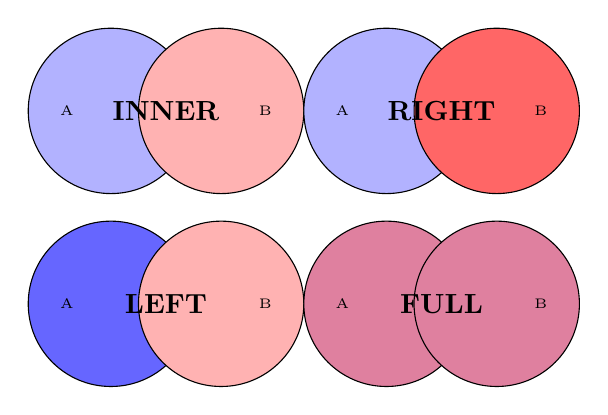
\begin{tikzpicture}[scale=0.7]
% Venn diagrams
\onslide<3->{
\draw[fill=blue!30] (0,0) circle (1.5cm);
\draw[fill=red!30] (2,0) circle (1.5cm);
\node at (1,0) {\textbf{INNER}};
\node at (-0.8,0) {\tiny A};
\node at (2.8,0) {\tiny B};
}

\onslide<4->{
\draw[fill=blue!60] (0,-3.5) circle (1.5cm);
\draw[fill=red!30] (2,-3.5) circle (1.5cm);
\node at (1,-3.5) {\textbf{LEFT}};
\node at (-0.8,-3.5) {\tiny A};
\node at (2.8,-3.5) {\tiny B};
}

\onslide<5->{
\draw[fill=blue!30] (5,0) circle (1.5cm);
\draw[fill=red!60] (7,0) circle (1.5cm);
\node at (6,0) {\textbf{RIGHT}};
\node at (4.2,0) {\tiny A};
\node at (7.8,0) {\tiny B};
}

\onslide<6->{
\draw[fill=purple!50] (5,-3.5) circle (1.5cm);
\draw[fill=purple!50] (7,-3.5) circle (1.5cm);
\node at (6,-3.5) {\textbf{FULL}};
\node at (4.2,-3.5) {\tiny A};
\node at (7.8,-3.5) {\tiny B};
}
\end{tikzpicture}
\end{column}
\end{columns}
\end{frame}

\begin{frame}[fragile]{INNER JOIN}
\begin{block}<1->{Definition}
Returns only rows that have matching values in both tables. Non-matching rows are excluded.
\end{block}

\pause
\begin{exampleblock}<2->{INNER JOIN Examples}
\begin{lstlisting}
-- Basic INNER JOIN
SELECT e.first_name, e.last_name, d.dept_name
FROM employees e
INNER JOIN departments d ON e.dept_id = d.dept_id;

-- Multiple INNER JOINs
SELECT e.first_name, d.dept_name, l.city
FROM employees e
INNER JOIN departments d ON e.dept_id = d.dept_id
INNER JOIN locations l ON d.location_id = l.location_id;

-- JOIN with WHERE clause
SELECT e.first_name, d.dept_name
FROM employees e
INNER JOIN departments d ON e.dept_id = d.dept_id
WHERE e.salary > 10000;

-- JOIN with table aliases
SELECT e.first_name, m.first_name AS manager_name
FROM employees e
INNER JOIN employees m ON e.manager_id = m.emp_id;
\end{lstlisting}
\end{exampleblock}
\end{frame}

\begin{frame}[fragile]{LEFT and RIGHT JOINs}
\begin{columns}[T]
\begin{column}{0.5\textwidth}
\onslide<1->{
\begin{block}{LEFT JOIN}
Returns all rows from the left table, and matching rows from the right table. Non-matching right table rows return NULL.
\end{block}

\begin{exampleblock}<2->{LEFT JOIN Examples}
\begin{lstlisting}
-- All employees with departments
SELECT e.first_name, d.dept_name
FROM employees e
LEFT JOIN departments d ON e.dept_id = d.dept_id;

-- Employees without departments
SELECT e.first_name
FROM employees e
LEFT JOIN departments d ON e.dept_id = d.dept_id
WHERE d.dept_id IS NULL;

-- Count employees per dept
SELECT d.dept_name, COUNT(e.emp_id) AS emp_count
FROM departments d
LEFT JOIN employees e ON d.dept_id = e.dept_id
GROUP BY d.dept_name;
\end{lstlisting}
\end{exampleblock}
}
\end{column}

\pause
\begin{column}{0.5\textwidth}
\begin{block}<3->{RIGHT JOIN}
Returns all rows from the right table, and matching rows from the left table. Non-matching left table rows return NULL.
\end{block}

\begin{exampleblock}<4->{RIGHT JOIN Example}
\begin{lstlisting}
-- All departments with employees
SELECT e.first_name, d.dept_name
FROM employees e
RIGHT JOIN departments d ON e.dept_id = d.dept_id;

-- Note: RIGHT JOIN is less common
-- Usually rewritten as LEFT JOIN
-- by swapping table order
\end{lstlisting}
\end{exampleblock}

\pause
\begin{alertblock}<5->{Best Practice}
Prefer LEFT JOIN over RIGHT JOIN for consistency. If you need a RIGHT JOIN, consider swapping the table order and using LEFT JOIN instead.
\end{alertblock}
\end{column}
\end{columns}
\end{frame}

\begin{frame}[fragile]{FULL OUTER JOIN and CROSS JOIN}
\begin{block}<1->{FULL OUTER JOIN}
Returns all rows when there is a match in either left or right table. Non-matching rows return NULL for the other table.
\end{block}

\pause
\begin{exampleblock}<2->{FULL OUTER JOIN}
\begin{lstlisting}
-- All employees and departments
SELECT e.first_name, d.dept_name
FROM employees e
FULL OUTER JOIN departments d ON e.dept_id = d.dept_id;

-- Note: MySQL doesn't support FULL OUTER JOIN
-- Workaround using UNION
SELECT e.first_name, d.dept_name
FROM employees e
LEFT JOIN departments d ON e.dept_id = d.dept_id
UNION
SELECT e.first_name, d.dept_name
FROM employees e
RIGHT JOIN departments d ON e.dept_id = d.dept_id;
\end{lstlisting}
\end{exampleblock}

\pause
\begin{block}<3->{CROSS JOIN}
Returns the Cartesian product of both tables (all combinations). Use with caution!
\end{block}

\pause
\begin{exampleblock}<4->{CROSS JOIN Example}
\begin{lstlisting}
-- All employee-department combinations
SELECT e.first_name, d.dept_name
FROM employees e
CROSS JOIN departments d;

-- Equivalent to:
SELECT e.first_name, d.dept_name
FROM employees e, departments d;
\end{lstlisting}
\end{exampleblock}
\end{frame}

\begin{frame}[fragile]{SELF JOIN and Advanced Joins}
\begin{block}<1->{SELF JOIN}
Joining a table to itself. Useful for hierarchical data.
\end{block}

\pause
\begin{exampleblock}<2->{SELF JOIN Examples}
\begin{lstlisting}
-- Employee with their manager
SELECT e.first_name AS employee, m.first_name AS manager
FROM employees e
LEFT JOIN employees m ON e.manager_id = m.emp_id;

-- Employees and their subordinates
SELECT m.first_name AS manager, COUNT(e.emp_id) AS num_subordinates
FROM employees m
LEFT JOIN employees e ON e.manager_id = m.emp_id
GROUP BY m.emp_id, m.first_name;

-- Hierarchical query (Oracle)
SELECT LEVEL, first_name, manager_id
FROM employees
START WITH manager_id IS NULL
CONNECT BY PRIOR emp_id = manager_id;
\end{lstlisting}
\end{exampleblock}
\end{frame}

\begin{frame}[fragile]{Join Conditions and Performance}
\begin{exampleblock}<1->{Different Join Syntaxes}
\begin{lstlisting}
-- ANSI SQL-92 (Recommended)
SELECT e.first_name, d.dept_name
FROM employees e
INNER JOIN departments d ON e.dept_id = d.dept_id;

-- ANSI SQL-89 (Old style)
SELECT e.first_name, d.dept_name
FROM employees e, departments d
WHERE e.dept_id = d.dept_id;

-- Multiple conditions
SELECT e.first_name, d.dept_name
FROM employees e
INNER JOIN departments d ON e.dept_id = d.dept_id
    AND e.hire_date > d.established_date;

-- USING shorthand (when column names match)
SELECT e.first_name, dept_name
FROM employees e
INNER JOIN departments USING (dept_id);
\end{lstlisting}
\end{exampleblock}

\pause
\begin{alertblock}<2->{Join Performance Tips}
\begin{itemize}
    \item Always use explicit JOIN syntax (ANSI SQL-92)
    \item Ensure joined columns are indexed
    \item Avoid joining on calculated columns
    \item Use appropriate join type (don't use OUTER when INNER suffices)
    \item Filter early in WHERE clause before joining
\end{itemize}
\end{alertblock}
\end{frame}

%=============================================================================
% PART 8: SUBQUERIES
%=============================================================================
\section{Subqueries}

\begin{frame}{Subquery Fundamentals}
\begin{block}<1->{Definition}
A \textbf{subquery} (or inner query) is a query nested inside another query (outer query). Subqueries can return:
\begin{itemize}
    \item A single value (scalar subquery)
    \item A single column (single-column subquery)
    \item Multiple columns (multi-column subquery)
    \item A table (table subquery)
\end{itemize}
\end{block}

\pause
\begin{block}<2->{Types of Subqueries}
\begin{itemize}
    \item \textbf{Correlated} - References outer query (executes once per row)
    \item \textbf{Non-correlated} - Independent of outer query (executes once total)
    \item \textbf{Scalar} - Returns exactly one value
    \item \textbf{Multi-row} - Returns multiple rows
\end{itemize}
\end{block}
\end{frame}

\begin{frame}[fragile]{Scalar Subqueries}
\begin{block}<1->{Definition}
Returns exactly one row with one column. Can be used anywhere a single value is expected.
\end{block}

\pause
\begin{exampleblock}<2->{Scalar Subquery Examples}
\begin{lstlisting}
-- Employees earning above average
SELECT first_name, salary
FROM employees
WHERE salary > (SELECT AVG(salary) FROM employees);

-- Employees in largest department
SELECT first_name
FROM employees
WHERE dept_id = (
    SELECT dept_id FROM employees 
    GROUP BY dept_id ORDER BY COUNT(*) DESC LIMIT 1
);

-- Subquery in SELECT clause
SELECT first_name, salary,
    (SELECT AVG(salary) FROM employees) AS avg_salary,
    salary - (SELECT AVG(salary) FROM employees) AS diff
FROM employees;
\end{lstlisting}
\end{exampleblock}
\end{frame}

\begin{frame}[fragile]{Multi-Row Subqueries}
\begin{block}<1->{Operators}
\begin{itemize}
    \item \texttt{IN} - Match any value in list
    \item \texttt{NOT IN} - Not match any value
    \item \texttt{ANY} / \texttt{SOME} - Compare to any value
    \item \texttt{ALL} - Compare to all values
    \item \texttt{EXISTS} - Check if subquery returns rows
\end{itemize}
\end{block}

\pause
\begin{exampleblock}<2->{Multi-Row Examples}
\begin{lstlisting}
-- IN operator
SELECT * FROM employees
WHERE dept_id IN (SELECT dept_id FROM departments WHERE location_id = 1700);

-- ANY operator
SELECT * FROM employees
WHERE salary > ANY (SELECT salary FROM employees WHERE dept_id = 30);

-- ALL operator
SELECT * FROM employees
WHERE salary > ALL (SELECT salary FROM employees WHERE dept_id = 30);

-- EXISTS
SELECT * FROM departments d
WHERE EXISTS (SELECT 1 FROM employees e WHERE e.dept_id = d.dept_id);
\end{lstlisting}
\end{exampleblock}
\end{frame}

\begin{frame}[fragile]{Correlated Subqueries}
\begin{block}<1->{Definition}
References columns from the outer query. Executes once for each row processed by the outer query.
\end{block}

\pause
\begin{exampleblock}<2->{Correlated Subquery Examples}
\begin{lstlisting}
-- Employees earning above their department average
SELECT e1.first_name, e1.salary, e1.dept_id
FROM employees e1
WHERE e1.salary > (
    SELECT AVG(e2.salary)
    FROM employees e2
    WHERE e2.dept_id = e1.dept_id
);

-- Departments with above-average salary
SELECT d.dept_name
FROM departments d
WHERE (SELECT AVG(salary) FROM employees e WHERE e.dept_id = d.dept_id) > 
      (SELECT AVG(salary) FROM employees);

-- EXISTS with correlation
SELECT e.first_name
FROM employees e
WHERE EXISTS (
    SELECT 1 FROM job_history jh WHERE jh.emp_id = e.emp_id
);
\end{lstlisting}
\end{exampleblock}
\end{frame}

\begin{frame}[fragile]{Subqueries in FROM Clause}
\begin{block}<1->{Derived Tables}
Subqueries in the FROM clause create temporary tables (derived tables) that can be used in the outer query.
\end{block}

\pause
\begin{exampleblock}<2->{Derived Table Examples}
\begin{lstlisting}
-- Average salary by department
SELECT d.dept_name, avg_sal.avg_salary
FROM departments d
INNER JOIN (
    SELECT dept_id, AVG(salary) AS avg_salary
    FROM employees
    GROUP BY dept_id
) avg_sal ON d.dept_id = avg_sal.dept_id;

-- Top 3 departments by average salary
SELECT dept_id, avg_salary
FROM (
    SELECT dept_id, AVG(salary) AS avg_salary
    FROM employees
    GROUP BY dept_id
) dept_avg
ORDER BY avg_salary DESC
LIMIT 3;

-- Multiple derived tables
SELECT e.dept_id, e.avg_sal, d.max_sal
FROM (SELECT dept_id, AVG(salary) AS avg_sal FROM employees GROUP BY dept_id) e
JOIN (SELECT dept_id, MAX(salary) AS max_sal FROM employees GROUP BY dept_id) d 
    ON e.dept_id = d.dept_id;
\end{lstlisting}
\end{exampleblock}
\end{frame}

%=============================================================================
% PART 9: SET OPERATIONS
%=============================================================================
\section{Set Operations}

\begin{frame}[fragile]{UNION, INTERSECT, and EXCEPT}
\begin{block}<1->{Set Operators}
Combine results from multiple SELECT statements:
\begin{itemize}
    \item \textbf{UNION} - Combine results, remove duplicates
    \item \textbf{UNION ALL} - Combine results, keep duplicates
    \item \textbf{INTERSECT} - Return common rows
    \item \textbf{EXCEPT/MINUS} - Return rows in first but not second
\end{itemize}
\end{block}

\pause
\begin{exampleblock}<2->{Set Operation Examples}
\begin{lstlisting}
-- UNION: All unique employee names from two tables
SELECT first_name FROM employees
UNION
SELECT first_name FROM former_employees;

-- UNION ALL: All names including duplicates
SELECT first_name FROM employees
UNION ALL
SELECT first_name FROM former_employees;

-- INTERSECT: Employees who are also managers
SELECT emp_id FROM employees
INTERSECT
SELECT manager_id FROM employees WHERE manager_id IS NOT NULL;

-- EXCEPT: Employees never in job history
SELECT emp_id FROM employees
EXCEPT
SELECT emp_id FROM job_history;
\end{lstlisting}
\end{exampleblock}
\end{frame}

\begin{frame}[fragile]{Set Operation Rules}
\begin{block}<1->{Requirements}
\begin{itemize}
    \item Same number of columns in both SELECTs
    \item Corresponding columns must have compatible data types
    \item Column names from first SELECT are used
    \item ORDER BY applies to final result
\end{itemize}
\end{block}

\pause
\begin{exampleblock}<2->{Advanced Set Operations}
\begin{lstlisting}
-- With ORDER BY (must be at end)
SELECT first_name, salary FROM employees WHERE dept_id = 10
UNION
SELECT first_name, salary FROM employees WHERE dept_id = 20
ORDER BY salary DESC;

-- Using column positions
SELECT first_name, salary FROM employees WHERE dept_id = 10
UNION
SELECT first_name, salary FROM employees WHERE dept_id = 20
ORDER BY 2 DESC;

-- Complex example with all three
(SELECT emp_id FROM employees WHERE salary > 10000)
UNION
(SELECT emp_id FROM job_history WHERE end_date IS NULL)
EXCEPT
(SELECT manager_id FROM employees WHERE manager_id IS NOT NULL);
\end{lstlisting}
\end{exampleblock}
\end{frame}

%=============================================================================
% PART 10: DML OPERATIONS
%=============================================================================
\section{Data Manipulation Language (DML)}

\begin{frame}[fragile]{INSERT Statements}
\begin{alertblock}{\textcolor{red}{\ding{43}} Safety First}<1->
Always verify your data before inserting. Use transactions for multiple inserts.
\end{alertblock}

\pause
\begin{exampleblock}<2->{INSERT Examples}
\begin{lstlisting}
-- Insert single row with all columns
INSERT INTO employees 
VALUES (207, 'John', 'Doe', 'john.doe@email.com', '555-0100', 
        '2024-01-15', 9, 5000, NULL, 100, 10);

-- Insert with specific columns
INSERT INTO employees (first_name, last_name, email, hire_date, job_id)
VALUES ('Jane', 'Smith', 'jane.smith@email.com', CURRENT_DATE, 9);

-- Insert multiple rows
INSERT INTO employees (first_name, last_name, email, hire_date)
VALUES 
    ('Alice', 'Johnson', 'alice@email.com', '2024-01-15'),
    ('Bob', 'Williams', 'bob@email.com', '2024-01-16'),
    ('Carol', 'Brown', 'carol@email.com', '2024-01-17');
\end{lstlisting}
\end{exampleblock}
\end{frame}

\begin{frame}[fragile]{INSERT with SELECT}
\begin{exampleblock}<1->{Insert from Another Table}
\begin{lstlisting}
-- Copy data from another table
INSERT INTO employees_backup
SELECT * FROM employees
WHERE hire_date < '2020-01-01';

-- Insert with column mapping
INSERT INTO employees_archive (emp_id, full_name, hire_date, termination_date)
SELECT emp_id, CONCAT(first_name, ' ', last_name), hire_date, CURRENT_DATE
FROM employees
WHERE termination_date IS NOT NULL;

-- Insert with subquery
INSERT INTO high_performers (emp_id, name, salary)
SELECT emp_id, CONCAT(first_name, ' ', last_name), salary
FROM employees
WHERE salary > (SELECT AVG(salary) * 1.5 FROM employees);
\end{lstlisting}
\end{exampleblock}

\pause
\begin{exampleblock}<2->{Database-Specific Features}
\begin{lstlisting}
-- MySQL: INSERT IGNORE (skip duplicates)
INSERT IGNORE INTO employees (emp_id, email)
VALUES (1, 'existing@email.com');

-- PostgreSQL: ON CONFLICT (upsert)
INSERT INTO employees (emp_id, email)
VALUES (1, 'new@email.com')
ON CONFLICT (emp_id) DO UPDATE SET email = EXCLUDED.email;

-- SQL Server: MERGE (upsert)
MERGE employees AS target
USING (VALUES (1, 'new@email.com')) AS source (emp_id, email)
ON target.emp_id = source.emp_id
WHEN MATCHED THEN UPDATE SET email = source.email
WHEN NOT MATCHED THEN INSERT (emp_id, email) VALUES (source.emp_id, source.email);
\end{lstlisting}
\end{exampleblock}
\end{frame}

\begin{frame}[fragile]{UPDATE Statements}
\begin{alertblock}{\textcolor{red}{\ding{43}} Critical Warning}<1->
\textbf{Always} use WHERE clause with UPDATE! Without it, you'll update ALL rows.
\end{alertblock}

\pause
\begin{exampleblock}<2->{UPDATE Examples}
\begin{lstlisting}
-- Update single column
UPDATE employees
SET salary = salary * 1.05
WHERE emp_id = 101;

-- Update multiple columns
UPDATE employees
SET salary = salary * 1.10, commission_pct = 0.15,
    last_modified = CURRENT_TIMESTAMP
WHERE dept_id = 80;

-- Update with subquery
UPDATE employees
SET salary = (
    SELECT AVG(salary) * 1.2
    FROM employees e2
    WHERE e2.dept_id = employees.dept_id
)
WHERE salary < (SELECT AVG(salary) FROM employees);
\end{lstlisting}
\end{exampleblock}
\end{frame}

\begin{frame}[fragile]{UPDATE with JOIN}
\begin{exampleblock}<1->{UPDATE with JOIN Examples}
\begin{lstlisting}
-- MySQL: UPDATE with JOIN
UPDATE employees e
INNER JOIN departments d ON e.dept_id = d.dept_id
SET e.salary = e.salary * 1.10
WHERE d.location_id = 1700;

-- PostgreSQL: UPDATE with FROM
UPDATE employees e
SET salary = salary * 1.10
FROM departments d
WHERE e.dept_id = d.dept_id AND d.location_id = 1700;

-- SQL Server: UPDATE with JOIN
UPDATE e
SET salary = salary * 1.10
FROM employees e
INNER JOIN departments d ON e.dept_id = d.dept_id
WHERE d.location_id = 1700;

-- Update with CASE
UPDATE employees
SET salary = CASE
    WHEN dept_id = 10 THEN salary * 1.05
    WHEN dept_id = 20 THEN salary * 1.10
    ELSE salary * 1.03
END;
\end{lstlisting}
\end{exampleblock}
\end{frame}

\begin{frame}[fragile]{DELETE Statements}
\begin{alertblock}{\textcolor{red}{\ding{43}} Critical Warning}<1->
\textbf{Always} use WHERE clause with DELETE! Without it, you'll delete ALL rows. Consider using transactions.
\end{alertblock}

\pause
\begin{exampleblock}<2->{DELETE Examples}
\begin{lstlisting}
-- Delete single row
DELETE FROM employees
WHERE emp_id = 999;

-- Delete with condition
DELETE FROM employees
WHERE hire_date < '2010-01-01'
AND termination_date IS NOT NULL;

-- Delete with subquery
DELETE FROM employees
WHERE dept_id IN (
    SELECT dept_id FROM departments
    WHERE location_id = 1700
);

-- Delete with JOIN (MySQL)
DELETE e FROM employees e
INNER JOIN departments d ON e.dept_id = d.dept_id
WHERE d.dept_name = 'Sales';

-- Delete with LIMIT (MySQL)
DELETE FROM employees
WHERE dept_id = 10
ORDER BY hire_date ASC
LIMIT 5;
\end{lstlisting}
\end{exampleblock}
\end{frame}

\begin{frame}[fragile]{MERGE Statement}
\begin{block}<1->{Definition}
\textbf{MERGE} (also called UPSERT) performs INSERT, UPDATE, or DELETE operations based on whether a row exists. Available in SQL Server, Oracle, PostgreSQL, and MySQL (as INSERT ... ON DUPLICATE KEY UPDATE).
\end{block}

\pause
\begin{exampleblock}<2->{MERGE Examples}
\begin{lstlisting}
-- SQL Server / Oracle
MERGE INTO employees AS target
USING (
    SELECT 101 AS emp_id, 'John Updated' AS first_name, 75000 AS salary
    UNION ALL
    SELECT 999, 'New Employee', 50000
) AS source ON target.emp_id = source.emp_id
WHEN MATCHED THEN
    UPDATE SET first_name = source.first_name, salary = source.salary
WHEN NOT MATCHED THEN
    INSERT (emp_id, first_name, salary) VALUES (source.emp_id, source.first_name, source.salary);

-- PostgreSQL
INSERT INTO employees (emp_id, first_name, salary)
VALUES (101, 'John Updated', 75000)
ON CONFLICT (emp_id) DO UPDATE SET first_name = EXCLUDED.first_name, salary = EXCLUDED.salary;

-- MySQL
INSERT INTO employees (emp_id, first_name, salary)
VALUES (101, 'John Updated', 75000)
ON DUPLICATE KEY UPDATE first_name = VALUES(first_name), salary = VALUES(salary);
\end{lstlisting}
\end{exampleblock}
\end{frame}

%=============================================================================
% PART 11: TRANSACTIONS
%=============================================================================
\section{Transactions}

\begin{frame}{Transaction Fundamentals}
\begin{block}<1->{ACID Properties}
\begin{itemize}
    \item \textbf{Atomicity} - All operations complete or none
    \item \textbf{Consistency} - Database remains in valid state
    \item \textbf{Isolation} - Concurrent transactions don't interfere
    \item \textbf{Durability} - Committed changes are permanent
\end{itemize}
\end{block}

\pause
\begin{block}<2->{Transaction Commands}
\begin{itemize}
    \item \texttt{BEGIN TRANSACTION} / \texttt{START TRANSACTION} - Begin transaction
    \item \texttt{COMMIT} - Save changes permanently
    \item \texttt{ROLLBACK} - Undo changes
    \item \texttt{SAVEPOINT} - Create savepoint within transaction
    \item \texttt{ROLLBACK TO SAVEPOINT} - Rollback to savepoint
\end{itemize}
\end{block}
\end{frame}

\begin{frame}[fragile]{Transaction Examples}
\begin{exampleblock}<1->{Basic Transaction}
\begin{lstlisting}
-- Transfer money between accounts
BEGIN TRANSACTION;

UPDATE accounts SET balance = balance - 1000 WHERE account_id = 'A123';
UPDATE accounts SET balance = balance + 1000 WHERE account_id = 'B456';

-- Check if both updates succeeded
IF @@ROWCOUNT = 2  -- SQL Server
    COMMIT;
ELSE
    ROLLBACK;
\end{lstlisting}
\end{exampleblock}

\pause
\begin{exampleblock}<2->{Savepoints}
\begin{lstlisting}
BEGIN TRANSACTION;

INSERT INTO orders (order_id, customer_id, order_date)
VALUES (1001, 'C001', CURRENT_DATE);

SAVEPOINT after_order_insert;

INSERT INTO order_items (order_id, product_id, quantity)
VALUES (1001, 'P001', 5);

-- If item insert fails, rollback to savepoint
ROLLBACK TO SAVEPOINT after_order_insert;

-- Continue with other operations
INSERT INTO order_items (order_id, product_id, quantity)
VALUES (1001, 'P002', 3);

COMMIT;
\end{lstlisting}
\end{exampleblock}
\end{frame}

\begin{frame}{Transaction Isolation Levels}
\begin{block}<1->{Isolation Levels}
\begin{center}
\begin{tabular}{llll}
\toprule
\textbf{Level} & \textbf{Dirty Read} & \textbf{Non-Repeatable} & \textbf{Phantom} \\
\midrule
READ UNCOMMITTED & Yes & Yes & Yes \\
READ COMMITTED & No & Yes & Yes \\
REPEATABLE READ & No & No & Yes \\
SERIALIZABLE & No & No & No \\
\bottomrule
\end{tabular}
\end{center}
\end{block}

\pause
\begin{exampleblock}<2->{Setting Isolation Level}
\begin{lstlisting}
-- SQL Server
SET TRANSACTION ISOLATION LEVEL SERIALIZABLE;
BEGIN TRANSACTION;

-- MySQL
SET SESSION TRANSACTION ISOLATION LEVEL READ COMMITTED;
START TRANSACTION;

-- Oracle (only READ COMMITTED and SERIALIZABLE)
SET TRANSACTION ISOLATION LEVEL SERIALIZABLE;

-- PostgreSQL
BEGIN TRANSACTION ISOLATION LEVEL REPEATABLE READ;
\end{lstlisting}
\end{exampleblock}
\end{frame}

%=============================================================================
% PART 12: VIEWS
%=============================================================================
\section{Views}

\begin{frame}[fragile]{Creating and Using Views}
\begin{block}<1->{Definition}
A \textbf{view} is a virtual table based on the result of a SQL query. It doesn't store data but provides a way to save complex queries for reuse.
\end{block}

\pause
\begin{exampleblock}<2->{Creating Views}
\begin{lstlisting}
-- Simple view
CREATE VIEW employee_details AS
SELECT e.emp_id, CONCAT(e.first_name, ' ', e.last_name) AS full_name,
       e.email, d.dept_name, l.city, e.salary
FROM employees e
JOIN departments d ON e.dept_id = d.dept_id
JOIN locations l ON d.location_id = l.location_id;

-- Query the view
SELECT * FROM employee_details WHERE city = 'Seattle';

-- View with check option
CREATE VIEW high_earners AS
SELECT * FROM employees WHERE salary > 10000
WITH CHECK OPTION;  -- Prevents inserting low salaries
\end{lstlisting}
\end{exampleblock}
\end{frame}

\begin{frame}[fragile]{Advanced Views}
\begin{exampleblock}<1->{Updatable Views}
\begin{lstlisting}
-- Simple updatable view
CREATE VIEW dept_10_employees AS
SELECT emp_id, first_name, last_name, salary
FROM employees
WHERE dept_id = 10;

-- Update through view
UPDATE dept_10_employees SET salary = salary * 1.05 WHERE emp_id = 101;

-- Insert through view
INSERT INTO dept_10_employees (emp_id, first_name, last_name, salary)
VALUES (999, 'New', 'Employee', 5000);  -- Must specify dept_id=10
\end{lstlisting}
\end{exampleblock}

\pause
\begin{exampleblock}<2->{Materialized Views}
\begin{lstlisting}
-- PostgreSQL / Oracle: Materialized view (stores data)
CREATE MATERIALIZED VIEW dept_summary AS
SELECT dept_id, COUNT(*) AS emp_count, AVG(salary) AS avg_salary
FROM employees
GROUP BY dept_id;

-- Refresh materialized view
REFRESH MATERIALIZED VIEW dept_summary;

-- Create with auto-refresh (PostgreSQL)
CREATE MATERIALIZED VIEW dept_summary AS
SELECT dept_id, COUNT(*) AS emp_count, AVG(salary) AS avg_salary
FROM employees
GROUP BY dept_id
WITH DATA;
\end{lstlisting}
\end{exampleblock}
\end{frame}

%=============================================================================
% PART 13: INDEXES
%=============================================================================
\section{Indexes}

\begin{frame}[fragile]{Creating Indexes}
\begin{block}<1->{Types of Indexes}
\begin{itemize}
    \item \textbf{B-Tree Index} - Default, good for equality and range
    \item \textbf{Hash Index} - Good for equality only
    \item \textbf{Bitmap Index} - Good for low cardinality
    \item \textbf{Full-text Index} - For text search
    \item \textbf{Spatial Index} - For geographic data
    \item \textbf{Composite Index} - Multiple columns
    \item \textbf{Unique Index} - Enforces uniqueness
\end{itemize}
\end{block}

\pause
\begin{exampleblock}<2->{Creating Indexes}
\begin{lstlisting}
-- Simple index
CREATE INDEX idx_emp_lastname ON employees(last_name);

-- Unique index
CREATE UNIQUE INDEX idx_emp_email ON employees(email);

-- Composite index
CREATE INDEX idx_emp_dept_salary ON employees(dept_id, salary);

-- Index with sorting
CREATE INDEX idx_emp_hiredate ON employees(hire_date DESC);

-- Partial index (PostgreSQL)
CREATE INDEX idx_high_earners ON employees(salary) WHERE salary > 10000;

-- Full-text index (MySQL)
CREATE FULLTEXT INDEX idx_description ON products(description);
\end{lstlisting}
\end{exampleblock}
\end{frame}

\begin{frame}[fragile]{Index Best Practices}
\begin{block}<1->{When to Create Indexes}
\begin{itemize}
    \item Columns frequently used in WHERE clauses
    \item Columns used in JOIN conditions
    \item Columns used in ORDER BY
    \item Columns with high selectivity (many unique values)
\end{itemize}
\end{block}

\pause
\begin{block}<2->{When NOT to Create Indexes}
\begin{itemize}
    \item Small tables (full scan is faster)
    \item Columns with few unique values (low cardinality)
    \item Columns frequently updated (maintenance overhead)
    \item Columns rarely queried
\end{itemize}
\end{block}

\pause
\begin{exampleblock}<3->{Index Maintenance}
\begin{lstlisting}
-- View query execution plan
EXPLAIN SELECT * FROM employees WHERE last_name = 'Smith';

-- Analyze table statistics
ANALYZE TABLE employees;

-- Rebuild index (SQL Server)
ALTER INDEX idx_emp_lastname ON employees REBUILD;

-- Drop index
DROP INDEX idx_emp_lastname ON employees;
\end{lstlisting}
\end{exampleblock}
\end{frame}

%=============================================================================
% PART 14: WINDOW FUNCTIONS
%=============================================================================
\section{Window Functions}

\begin{frame}{Window Function Fundamentals}
\begin{block}<1->{Definition}
\textbf{Window functions} perform calculations across a set of rows related to the current row (the "window"). Unlike aggregate functions, they don't collapse rows.
\end{block}

\pause
\begin{block}<2->{Types of Window Functions}
\begin{itemize}
    \item \textbf{Ranking}: ROW_NUMBER(), RANK(), DENSE_RANK(), NTILE()
    \item \textbf{Aggregate}: SUM(), AVG(), COUNT(), MIN(), MAX() over window
    \item \textbf{Analytic}: LAG(), LEAD(), FIRST_VALUE(), LAST_VALUE()
    \item \textbf{Statistical}: PERCENT_RANK(), CUME_DIST(), etc.
\end{itemize}
\end{block}

\pause
\begin{block}<3->{Syntax}
\begin{lstlisting}
function_name(expression) OVER (
    [PARTITION BY partition_column]
    [ORDER BY order_column]
    [frame_clause]
) AS alias
\end{lstlisting}
\end{block}
\end{frame}

\begin{frame}[fragile]{Ranking Functions}
\begin{exampleblock}<1->{ROW_NUMBER, RANK, DENSE_RANK}
\begin{lstlisting}
-- ROW_NUMBER: Unique sequential number
SELECT first_name, salary,
    ROW_NUMBER() OVER (ORDER BY salary DESC) AS row_num
FROM employees;

-- RANK: Same rank for ties, skips numbers
SELECT first_name, salary,
    RANK() OVER (ORDER BY salary DESC) AS rank_num
FROM employees;

-- DENSE_RANK: Same rank for ties, no gaps
SELECT first_name, salary,
    DENSE_RANK() OVER (ORDER BY salary DESC) AS dense_rank_num
FROM employees;

-- NTILE: Divide into buckets
SELECT first_name, salary,
    NTILE(4) OVER (ORDER BY salary DESC) AS quartile
FROM employees;
\end{lstlisting}
\end{exampleblock}
\end{frame}

\begin{frame}[fragile]{Ranking with PARTITION}
\begin{exampleblock}<1->{Partitioned Rankings}
\begin{lstlisting}
-- Rank within each department
SELECT first_name, dept_id, salary,
    RANK() OVER (PARTITION BY dept_id ORDER BY salary DESC) AS dept_rank
FROM employees;

-- Top 3 earners per department
WITH ranked_employees AS (
    SELECT first_name, dept_id, salary,
        ROW_NUMBER() OVER (PARTITION BY dept_id ORDER BY salary DESC) AS rn
    FROM employees
)
SELECT * FROM ranked_employees WHERE rn <= 3;

-- Percentile ranking
SELECT first_name, salary,
    PERCENT_RANK() OVER (ORDER BY salary) AS percentile
FROM employees;
\end{lstlisting}
\end{exampleblock}
\end{frame}

\begin{frame}[fragile]{Analytic Functions}
\begin{exampleblock}<1->{LAG and LEAD}
\begin{lstlisting}
-- LAG: Access previous row
SELECT emp_id, first_name, salary,
    LAG(salary, 1) OVER (ORDER BY hire_date) AS prev_salary,
    salary - LAG(salary, 1) OVER (ORDER BY hire_date) AS salary_diff
FROM employees;

-- LEAD: Access next row
SELECT emp_id, first_name, hire_date,
    LEAD(hire_date, 1) OVER (ORDER BY hire_date) AS next_hire_date,
    DATEDIFF(LEAD(hire_date) OVER (ORDER BY hire_date), hire_date) AS days_between
FROM employees;

-- LAG with default value
SELECT first_name, salary,
    LAG(salary, 1, 0) OVER (ORDER BY hire_date) AS prev_salary
FROM employees;
\end{lstlisting}
\end{exampleblock}
\end{frame}

\begin{frame}[fragile]{Aggregate Window Functions}
\begin{exampleblock}<1->{Running Totals and Moving Averages}
\begin{lstlisting}
-- Running total
SELECT first_name, salary,
    SUM(salary) OVER (ORDER BY hire_date) AS running_total
FROM employees;

-- Moving average (3-row window)
SELECT first_name, salary,
    AVG(salary) OVER (ORDER BY hire_date ROWS BETWEEN 2 PRECEDING AND CURRENT ROW) AS moving_avg
FROM employees;

-- Department total vs company total
SELECT first_name, dept_id, salary,
    SUM(salary) OVER (PARTITION BY dept_id) AS dept_total,
    SUM(salary) OVER () AS company_total,
    ROUND(salary * 100.0 / SUM(salary) OVER (PARTITION BY dept_id), 2) AS pct_of_dept
FROM employees;
\end{lstlisting}
\end{exampleblock}
\end{frame}

\begin{frame}[fragile]{Window Frames}
\begin{block}<1->{Frame Clauses}
\begin{itemize}
    \item \texttt{ROWS} - Physical row offset
    \item \texttt{RANGE} - Logical value offset
    \item \texttt{UNBOUNDED PRECEDING} - All rows before current
    \item \texttt{UNBOUNDED FOLLOWING} - All rows after current
    \item \texttt{CURRENT ROW} - Current row only
    \item \texttt{n PRECEDING/FOLLOWING} - n rows before/after
\end{itemize}
\end{block}

\pause
\begin{exampleblock}<2->{Frame Examples}
\begin{lstlisting}
-- Cumulative sum (all previous rows)
SUM(salary) OVER (ORDER BY hire_date ROWS UNBOUNDED PRECEDING)

-- 3-row moving average
AVG(salary) OVER (ORDER BY hire_date ROWS BETWEEN 1 PRECEDING AND 1 FOLLOWING)

-- First value in partition
FIRST_VALUE(salary) OVER (PARTITION BY dept_id ORDER BY hire_date)

-- Last value (requires frame)
LAST_VALUE(salary) OVER (PARTITION BY dept_id ORDER BY hire_date
    ROWS BETWEEN CURRENT ROW AND UNBOUNDED FOLLOWING)
\end{lstlisting}
\end{exampleblock}
\end{frame}

%=============================================================================
% PART 15: CTES
%=============================================================================
\section{Common Table Expressions (CTEs)}

\begin{frame}[fragile]{Basic CTEs}
\begin{block}<1->{Definition}
A \textbf{Common Table Expression (CTE)} is a temporary named result set that exists for the duration of a single query. Defined using the \texttt{WITH} clause.
\end{block}

\pause
\begin{exampleblock}<2->{Simple CTE Examples}
\begin{lstlisting}
-- Basic CTE
WITH high_earners AS (
    SELECT * FROM employees WHERE salary > 10000
)
SELECT first_name, salary FROM high_earners;

-- Multiple CTEs
WITH dept_avg AS (
    SELECT dept_id, AVG(salary) AS avg_sal FROM employees GROUP BY dept_id
),
company_avg AS (
    SELECT AVG(salary) AS avg_sal FROM employees
)
SELECT d.dept_id, d.avg_sal, c.avg_sal AS company_avg
FROM dept_avg d, company_avg c;

-- CTE with parameters (PostgreSQL)
WITH params AS (SELECT 10000 AS min_salary)
SELECT * FROM employees e, params p WHERE e.salary > p.min_salary;
\end{lstlisting}
\end{exampleblock}
\end{frame}

\begin{frame}[fragile]{Recursive CTEs}
\begin{block}<1->{Definition}
\textbf{Recursive CTEs} reference themselves, useful for hierarchical data (org charts, bill of materials, etc.).
\end{block}

\pause
\begin{exampleblock}<2->{Recursive CTE Example}
\begin{lstlisting}
-- Employee hierarchy
WITH RECURSIVE employee_hierarchy AS (
    -- Anchor member: top-level managers
    SELECT emp_id, first_name, manager_id, 0 AS level,
        CAST(first_name AS VARCHAR(1000)) AS path
    FROM employees
    WHERE manager_id IS NULL
    
    UNION ALL
    
    -- Recursive member: employees with managers
    SELECT e.emp_id, e.first_name, e.manager_id, eh.level + 1,
        eh.path || ' -> ' || e.first_name
    FROM employees e
    INNER JOIN employee_hierarchy eh ON e.manager_id = eh.emp_id
)
SELECT REPEAT('  ', level) || first_name AS org_chart, level, path
FROM employee_hierarchy
ORDER BY path;
\end{lstlisting}
\end{exampleblock}
\end{frame}

%=============================================================================
% PART 16: ADVANCED TOPICS
%=============================================================================
\section{Advanced Topics}

\begin{frame}[fragile]{Pivoting Data}
\begin{exampleblock}<1->{PIVOT (SQL Server / Oracle)}
\begin{lstlisting}
-- Convert rows to columns
SELECT *
FROM (
    SELECT dept_id, job_id, salary FROM employees
) AS source
PIVOT (
    AVG(salary)
    FOR job_id IN ([9], [10], [11])
) AS pivot_table;
\end{lstlisting}
\end{exampleblock}

\pause
\begin{exampleblock}<2->{Crosstab with CASE (Standard SQL)}
\begin{lstlisting}
-- Manual pivot using CASE
SELECT dept_id,
    SUM(CASE WHEN job_id = 9 THEN salary END) AS job_9_salary,
    SUM(CASE WHEN job_id = 10 THEN salary END) AS job_10_salary,
    SUM(CASE WHEN job_id = 11 THEN salary END) AS job_11_salary,
    COUNT(*) AS total_employees
FROM employees
GROUP BY dept_id;

-- UNPIVOT (reverse operation)
SELECT dept_id, job_type, salary
FROM (
    SELECT dept_id, job_9, job_10, job_11 FROM pivot_table
) p
UNPIVOT (salary FOR job_type IN (job_9, job_10, job_11)) AS unpvt;
\end{lstlisting}
\end{exampleblock}
\end{frame}

\begin{frame}[fragile]{Grouping Sets and Rollup}
\begin{exampleblock}<1->{GROUPING SETS}
\begin{lstlisting}
-- Multiple grouping levels in one query
SELECT dept_id, job_id, COUNT(*) AS emp_count
FROM employees
GROUP BY GROUPING SETS (
    (dept_id, job_id),  -- By dept and job
    (dept_id),          -- By dept only
    (job_id),           -- By job only
    ()                  -- Grand total
);
\end{lstlisting}
\end{exampleblock}

\pause
\begin{exampleblock}<2->{ROLLUP and CUBE}
\begin{lstlisting}
-- ROLLUP: hierarchical subtotals
SELECT dept_id, job_id, SUM(salary) AS total_salary
FROM employees
GROUP BY ROLLUP (dept_id, job_id);
-- Produces: (dept, job), (dept), ()

-- CUBE: all combinations
SELECT dept_id, job_id, SUM(salary) AS total_salary
FROM employees
GROUP BY CUBE (dept_id, job_id);
-- Produces: (dept, job), (dept), (job), ()

-- GROUPING function
SELECT COALESCE(dept_id, 'All Depts') AS dept, COALESCE(job_id, 'All Jobs') AS job,
    SUM(salary), GROUPING(dept_id) AS is_dept_total
FROM employees
GROUP BY ROLLUP (dept_id, job_id);
\end{lstlisting}
\end{exampleblock}
\end{frame}

\begin{frame}[fragile]{JSON and XML Support}
\begin{exampleblock}<1->{JSON Functions (PostgreSQL / MySQL / SQL Server)}
\begin{lstlisting}
-- Create JSON
SELECT JSON_OBJECT('name', first_name, 'salary', salary) FROM employees;

-- Aggregate to JSON array
SELECT dept_id, JSON_ARRAYAGG(JSON_OBJECT('name', first_name, 'salary', salary)) AS employees
FROM employees
GROUP BY dept_id;

-- Query JSON
SELECT * FROM employees WHERE JSON_EXTRACT(data, '$.department') = 'Sales';

-- Update JSON
UPDATE employees SET data = JSON_SET(data, '$.salary', 50000) WHERE emp_id = 101;
\end{lstlisting}
\end{exampleblock}

\pause
\begin{exampleblock}<2->{XML Functions}
\begin{lstlisting}
-- SQL Server: FOR XML
SELECT first_name, salary FROM employees FOR XML AUTO, ELEMENTS;

-- Oracle: XML functions
SELECT XMLELEMENT("Employee", XMLFOREST(first_name, salary)) FROM employees;
\end{lstlisting}
\end{exampleblock}
\end{frame}

%=============================================================================
% PART 17: PERFORMANCE
%=============================================================================
\section{Performance Optimization}

\begin{frame}[fragile]{Query Optimization}
\begin{block}<1->{Best Practices}
\begin{itemize}
    \item Use EXPLAIN to analyze query plans
    \item Select only needed columns (avoid SELECT *)
    \item Use appropriate indexes
    \item Filter early with WHERE clauses
    \item Use JOINs instead of subqueries when possible
    \item Avoid functions on indexed columns in WHERE
    \item Use LIMIT for testing large queries
\end{itemize}
\end{block}

\pause
\begin{exampleblock}<2->{EXPLAIN Examples}
\begin{lstlisting}
-- MySQL
EXPLAIN SELECT * FROM employees WHERE last_name = 'Smith';
EXPLAIN ANALYZE SELECT * FROM employees WHERE last_name = 'Smith';

-- PostgreSQL
EXPLAIN (ANALYZE, BUFFERS) SELECT * FROM employees WHERE last_name = 'Smith';

-- SQL Server
SET SHOWPLAN_XML ON;
SELECT * FROM employees WHERE last_name = 'Smith';

-- Oracle
EXPLAIN PLAN FOR SELECT * FROM employees WHERE last_name = 'Smith';
SELECT * FROM TABLE(DBMS_XPLAN.DISPLAY);
\end{lstlisting}
\end{exampleblock}
\end{frame}

\begin{frame}{Query Optimization Tips}
\begin{columns}[T]
\begin{column}{0.5\textwidth}
\onslide<1->{
\begin{block}{DO's}
\begin{itemize}
    \item Use parameterized queries
    \item Use appropriate data types
    \item Use EXISTS instead of IN for large subqueries
    \item Use UNION ALL instead of UNION when possible
    \item Use covering indexes
    \item Batch large updates
    \item Use connection pooling
\end{itemize}
\end{block}
}
\end{column}

\pause
\begin{column}{0.5\textwidth}
\begin{block}<2->{DON'Ts}
\begin{itemize}
    \item Use SELECT * in production
    \item Use cursors when set-based works
    \item Use functions on indexed columns
    \item Use implicit conversions
    \item Use OR on different columns
    \item Use NOT IN with NULL values
    \item Use wildcards at start of LIKE
\end{itemize}
\end{block}
\end{column}
\end{columns}

\pause
\begin{alertblock}<3->{Common Anti-Patterns}
\begin{itemize}
    \item \texttt{WHERE YEAR(date_column) = 2024} - Use range instead
    \item \texttt{WHERE column LIKE '%text'} - Can't use index
    \item \texttt{WHERE column = @var OR @var IS NULL} - Use dynamic SQL
    \item \texttt{SELECT DISTINCT} to fix duplicates - Fix the JOIN instead
\end{itemize}
\end{alertblock}
\end{frame}

%=============================================================================
% PART 18: QUICK REFERENCE
%=============================================================================
\section{Quick Reference}

\begin{frame}{SQL Quick Reference Card}
\begin{columns}[T]
\begin{column}{0.33\textwidth}
\onslide<1->{
\textbf{Query Order:}
\begin{enumerate}
    \item FROM
    \item WHERE
    \item GROUP BY
    \item HAVING
    \item SELECT
    \item DISTINCT
    \item ORDER BY
    \item LIMIT
\end{enumerate}

\vspace{0.5cm}
\textbf{Joins:}
\begin{itemize}
    \item INNER JOIN
    \item LEFT JOIN
    \item RIGHT JOIN
    \item FULL JOIN
    \item CROSS JOIN
\end{itemize}
}
\end{column}

\pause
\begin{column}{0.33\textwidth}
\textbf{Aggregates:}
\begin{itemize}
    \item COUNT(*)
    \item SUM()
    \item AVG()
    \item MAX()
    \item MIN()
\end{itemize}

\vspace{0.5cm}
\textbf{String:}
\begin{itemize}
    \item CONCAT()
    \item UPPER()/LOWER()
    \item SUBSTRING()
    \item LENGTH()
    \item TRIM()
    \item LIKE '%_'
\end{itemize}
\end{column}

\pause
\begin{column}{0.33\textwidth}
\textbf{Window:}
\begin{itemize}
    \item ROW_NUMBER()
    \item RANK()
    \item LAG()/LEAD()
    \item SUM() OVER()
    \item PARTITION BY
\end{itemize}

\vspace{0.5cm}
\textbf{Conditions:}
\begin{itemize}
    \item = <> < > <= >=
    \item BETWEEN
    \item IN / NOT IN
    \item IS NULL
    \item LIKE
    \item AND OR NOT
\end{itemize}
\end{column}
\end{columns}
\end{frame}

%=============================================================================
% FINAL SLIDE
%=============================================================================
\begin{frame}
\centering
\Huge Questions? \\[1cm]
\large Practice Exercises:
\normalsize
\begin{itemize}
    \item Find employees who earn more than their managers
    \item Calculate running total salary by department
    \item Find the second highest salary in each department
    \item Create a pivot table showing salary by department and job
    \item Write a recursive query to show full org chart
    \item Optimize a slow query using appropriate indexes
\end{itemize}
\end{frame}

\end{document}
